%===================================================================================
% JORNADA CIENTÍFICA ESTUDIANTIL - MATCOM, UH
%===================================================================================
% Esta plantilla ha sido diseñada para ser usada en los artículos de la
% Jornada Científica Estudiantil, MatCom.
%
% Por favor, siga las instrucciones de esta plantilla y rellene en las secciones
% correspondientes.
%
% NOTA: Necesitará el archivo 'jcematcom.sty' en la misma carpeta donde esté este
%       archivo para poder utilizar esta plantila.
%===================================================================================



%===================================================================================
% PREÁMBULO
%-----------------------------------------------------------------------------------
\documentclass[a4paper,10pt,twocolumn]{article}

%===================================================================================
% Paquetes
%-----------------------------------------------------------------------------------
\usepackage{amsmath}
\usepackage{amsfonts}
\usepackage{amssymb}
\usepackage{jcematcom}
\usepackage[utf8]{inputenc}
\usepackage{listings}
\usepackage[pdftex]{hyperref}

\usepackage{algorithm}
%\usepackage{algorithmic}

\usepackage{algpseudocode}
\usepackage[spanish]{babel}

%\usepackage[]{algorithm2e}
%-----------------------------------------------------------------------------------
% Configuración
%-----------------------------------------------------------------------------------
\hypersetup{colorlinks,%
	    citecolor=black,%
	    filecolor=black,%
	    linkcolor=black,%
	    urlcolor=blue}

%===================================================================================



%===================================================================================
% Presentacion
%-----------------------------------------------------------------------------------
% Título
%-----------------------------------------------------------------------------------
\title{Modelos de Optimización II \\
	Al desperdicio, ¡ni un tantico así!}

%-----------------------------------------------------------------------------------
% Autores
%-----------------------------------------------------------------------------------
\author{\\
\name Dalianys Pérez Pereira \email \href{mailto:d.perez3@estudiantes.matcom.uh.cu}{d.perez3@estudiantes.matcom.uh.cu}
	\\ \addr Grupo C411 \AND
\name Dayany Alfaro González \email \href{mailto:d.alfaro@estudiantes.matcom.uh.cu}{d.alfaro@estudiantes.matcom.uh.cu}
  \\ \addr Grupo C411 \AND
\name Gilberto González Rodríguez \email \href{mailto:mailto:g.gonzalez@estudiantes.matcom.uh.cu}{g.gonzalez@estudiantes.matcom.uh.cu}
\\ \addr Grupo C411 \AND
\name Antonio Jesús Otaño Barrera \email \href{mailto:a.otano@estudiantes.matcom.uh.cu}{a.otano@estudiantes.matcom.uh.cu}
\\ \addr Grupo C411}

%-----------------------------------------------------------------------------------
% Tutores
%-----------------------------------------------------------------------------------
%\tutors{\\
%Dr. Tutor Uno, \emph{Centro} \\
%Lic. Tutor Dos, \emph{Centro}}

%-----------------------------------------------------------------------------------
% Headings
%-----------------------------------------------------------------------------------
%\jcematcomheading{\the\year}{1-\pageref{end}}{A. Uno, A. Dos}

%-----------------------------------------------------------------------------------
%\ShortHeadings{Autores}
%===================================================================================



%===================================================================================
% DOCUMENTO
%-----------------------------------------------------------------------------------
\begin{document}
\begin{hyphenrules}{nohyphenation}
%-----------------------------------------------------------------------------------
% NO BORRAR ESTA LINEA!
%-----------------------------------------------------------------------------------
\twocolumn[
%-----------------------------------------------------------------------------------

\maketitle

%===================================================================================
% Resumen y Abstract
%-----------------------------------------------------------------------------------

\selectlanguage{spanish} % Para producir el documento en Español

%-----------------------------------------------------------------------------------
% Resumen en Español
%-----------------------------------------------------------------------------------
\begin{abstract}

Este trabajo tiene como objetivo resolver un problema de corte en dos dimensiones, asociado a la industria del papel, presente en la empresa GeoCuba ubicada en la provinicia Pinar del Río, Cuba. Se propone el  diseño e implementación de un algoritmo que permita determinar qué patrones de corte deben usarse para cortar un conjunto de hojas de forma que se satisfaga una demanda (de hojas más pequeñas) solicitada por el usuario de forma que el desperdicio resultante de los cortes sea el menor posible. En este caso se permite la rotación de las piezas a colocar y se requiere que los cortes sean de tipo guillotina. La solución que se propone se basa en un problema de programación lineal, un problema de empaquetamiento y un algoritmo génetico.

\end{abstract}

%-----------------------------------------------------------------------------------
% English Abstract
%-----------------------------------------------------------------------------------
\vspace{0.5cm}

\begin{enabstract}

This paper aims to solve a two-dimensional cutting stock problem associated with the paper industry, that was presented by the GeoCuba company located in Pinar del Río, Cuba. Here are proposed the design and implementation of an algorithm that allows determining which cutting patterns should be used to cut a set of sheets in such a way that a demand (for smaller sheets) requested by the user is satisfied so that the waste resulting from the cuts be the smallest possible. In this case, the rotation of the pieces to be placed is allowed and the cuts are required to be of the guillotine type. The proposed solution is based on a linear programming problem, a bin packing problem, and a genetic algorithm. 

\end{enabstract}

%-----------------------------------------------------------------------------------
% Palabras clave
%-----------------------------------------------------------------------------------
\begin{keywords}
	Problema de Patrones de Corte en dos dimensiones,
	Problema de Empaquetamiento en dos dimensiones,
	Algoritmo Genético,
	Industria del Papel.
\end{keywords}

%-----------------------------------------------------------------------------------
% Temas
%-----------------------------------------------------------------------------------
%\begin{topics}
%	Tema, Subtema.
%\end{topics}


%-----------------------------------------------------------------------------------
% NO BORRAR ESTAS LINEAS!
%-----------------------------------------------------------------------------------
\vspace{0.8cm}
]
%-----------------------------------------------------------------------------------


%===================================================================================

%===================================================================================
% Introducción
%-----------------------------------------------------------------------------------
\section{Introducción}\label{sec:intro}
%-----------------------------------------------------------------------------------
El problema de patrones de corte de piezas rectangulares pertenece a
la familia de problemas de corte y empaquetamiento y sus
aplicaciones se pueden observar en industrias de perfiles
metálicos, corte de maderas, papel, plástico o vidrio en
donde los componentes rectangulares tienen que ser
cortados de grandes hojas de material. Para estas industrias es de gran importancia realizar
este proceso de corte de una manera eficiente buscando
minimizar el desperdicio y los demás costos asociados
al proceso, teniendo en cuenta las restricciones técnicas
y de demanda. 



El problema de patrones de corte es un problema de gran
complejidad tanto por las características y variables
que involucra como por las técnicas que se utilizan
para abordarlo, es una temática en constante evolución
y muchos investigadores han desarrollado diversos
modelos para resolverlo. El interés en este problema
puede ser sustentado por su aplicación práctica y el
reto que representa, pues, en general,
es computacionalmente difícil de resolver ya que es un
problema de tipo NP-completo, dado que los patrones de
empaquetamiento incrementan exponencialmente con el
número de rectángulos que deben ser empaquetados. 
 
Este trabajo tiene como objetivo resolver un problema de corte en dos dimensiones, asociado a la industria del papel, presente en la empresa GeoCuba ubicada en la provinicia Pinar del Río, Cuba. Se propone el  diseño e implementación de un algoritmo que permita determinar qué patrones de corte deben usarse para cortar un conjunto de hojas de forma que se satisfaga una demanda (de hojas más pequeñas) solicitada por el usuario de forma que el desperdicio resultante de los cortes sea el menor posible. En este caso se permite la rotación de las piezas a colocar y se requiere que los cortes sean de tipo guillotina, es decir, que  el corte, ya sea horizontal o vertical, vaya de un extremo a otro de la hoja a picar y que a su vez produzca dos nuevas hojas que satisfagan este tipo de corte. 

La solución propuesta está implementada haciendo uso de Python como lenguaje. Además se brinda como parte de la solución una aplicación de escritorio con una interfaz de usuario para introducir una instancia del problema en cuestión. 

En la Sección \ref{estadodelarte} se abordan las principales aproximaciones al problema en cuestión que se han realizado hasta el momento. En la Sección \ref{def} se encuentra la definición formal del problema, mientras que la Sección \ref{prop} describe la solución propuesta en este trabajo. Por último la Sección \ref{visual} aborda detalles acerca de la interfaz visual que se provee para hacer uso de la presente solución.

%===================================================================================

\section{Antecedentes y Enfoques de Solución}\label{estadodelarte}
El Problema de patrones de corte (CSP, por sus siglas
en inglés) fue formulado por primera vez en 1939
por el economista ruso Kantorovich.

Han surgido numerosas investigaciones que abordan
diferentes problemas según el tipo de dimensión (1D y
2D) y desde diversos enfoques tales como los métodos
exactos, heurísticos y meta heurísticos, pero aún no
existe un método global establecido para dar solución
a este tipo de problemas, debido a la complejidad
asociada. 

\subsection{Programación Lineal Entera}

Casi todos los procedimientos basados en la
programación lineal para resolver el problema de
patrones de corte se remontan a Gilmore y Gomory,
\cite{1}, para lo cual, proponen la relajación de la restricción
de integridad para la solución de problemas de
programación lineal logrando minimizar el desperdicio
a través de la generación de columnas evitando el
conocimiento explícito o enumeración de todos los
patrones desde el principio, ya que bajo este esquema
las columnas (patrones) son generadas cuando se
requieran \cite{2}. La idea consiste en utilizar el método
simplex revisado para resolver el problema de la entrada
del patrón de corte siguiente a la base mediante la
resolución de un problema de la mochila asociado. Este
método es denominado en la literatura como \textit{delayed
column generation technique}, y permite resolver este
tipo de problemas en un tiempo computacional mucho
menor \cite{3}.


\subsection{Procedimientos Heurísticos Secuenciales}
Los procedimientos heurísticos secuenciales pertenecen
a la clase de heurísticas de búsqueda local. La solución
se construye mediante la generación de patrones uno
a uno hasta que todos los requerimientos de demanda
se hayan satisfecho, donde los patrones inicialmente
seleccionados deben tener un nivel de desperdicio
bajo, un nivel de utilización alto y dejar una serie de requerimientos para poder combinar bien los patrones
futuros, evitando así incurrir posteriormente en
desperdicios excesivos \cite{3}. La ventaja principal de este método es que puede controlar otros factores aparte del desperdicio y elimina
el problema del redondeo al trabajar sólo con valores
enteros.

\subsection{Procedimientos Heurísticos Híbridos }
Este procedimiento consiste en combinar los dos
procedimientos descritos anteriormente, de tal forma
que se utilice el procedimiento heurístico secuencial
para generar una solución, la cual es guardada y
utilizada como base inicial en el procedimiento de
programación lineal. Posteriormente, el desperdicio es
reducido si es posible a través iteraciones adicionales,
tal y como lo realiza \cite{41}. 

Independientemente de la forma como
se combinen estos dos métodos, lo más importante
del éxito de la unión entre el procedimiento heurístico
secuencial y el redondeo de problemas de programación
lineal es la selección del criterio apropiado para resolver
el problema \cite{29}.

\subsection{ Metaheurísticas }
Ante el problema que presenta la búsqueda local y
las heurísticas constructivas de quedar atrapadas en
óptimos locales, surgen las metaheurísticas a mediados
de 1970 pues tienen la capacidad de guiar la búsqueda
local para que se escape de los óptimos locales. Muchos
de estos algoritmos se han utilizado para resolver
el problema de patrones de corte, entre los cuales
se destaca \textit{Tabu Search} (TS), \textit{Greedy Randomized
Adaptive Search Procedure} (GRASP) \cite{42}, Algoritmos
genéticos \cite{43,46} y \textit{Ant Colony Optimization} (ACO) \cite{47,48}, entre otros algoritmos evolucionarios \cite{51}.

%===================================================================================
% Desarrollo
%-----------------------------------------------------------------------------------
\section{Definición del Problema}\label{def}
Sea $I$ el conjunto de $n$ hojas, una hoja $i$ está definida por su ancho $w_i$, su altura $h_i$ y su demanda $d_i$. Sea $J$ el conjunto de $m$ patrones de corte con las mismas dimensiones $H \times W$, el número $m$ es desconocido. Sea $p_{ji}$ el número de hojas $i$ presentes en el patrón $j$, se tiene que $p_j = (p_{j1},...,p_{jn})$. Sea $\pi_j$ una configuración de las hojas del patrón $j$, la cual incluye información acerca de la posición exacta de las hojas y si se encuentran rotadas o no. Por tanto, un patrón $j$ va a estar definido por $(p_j,\pi_j)$. Sea $x_j$ el número de veces que es necesario aplicar el patrón de corte $j$, se tiene que las variables de decisión son: $m, p_j, x_j$ y $\pi_j$ $\forall j \in J$.  

El objetivo que se persigue es minimizar el desperdicio de papel:
\begin{equation}
f = \sum_{j \in J}c_j x_j
\label{eq1}
\end{equation}
donde $c_j$ es el área no usada del patrón $j$.

Para satisfacer la demanda $d_i$ solicitada para cada hoja $i$ van a aparecer $n$ restricciones:
\begin{equation}
\sum_{j \in J}p_{ji}x_j \geq  d_i \ \  \forall i \in I
\label{eq2}
\end{equation}

Es necesario también tener en cuenta la sobreproducción a la hora de analizar el espacio desperdiciado dado que cuando una solución sobrecumple la demanda se tiene que esas hojas sobreproducidas también van a ser desechadas. Por tanto para tener lo anterior en consideración hay que modificar la función objetivo que se muestra en la Ecuación \eqref{eq1}. Sea $a_i$ el área total de la hoja $i$, se tiene que:
 $$sobreProd = \sum_{i \in I} sobreProd_i $$ 
donde $sobreProd_i = (\sum_{j \in J} p_{ji}x_ja_i)  -  d_ia_i$ va a ser el área total que ocupa la sobreproducción de hoja de tipo $i$ sobreproducidas.
La nueva función objetivo sería la siguiente:
\begin{equation}
f = \sum_{j \in J}c_j x_j + sobreProd
\label{eq3}
\end{equation}

Esta función objetivo y las $n$ restricciones presentadas antes definen un problema de programación lineal entero. Sea $S$ el conjunto de todas las posibles soluciones, una solución $s \in S$ va a estar formada por $((p_1,\pi_1),...,(p_m,\pi_m))$ y $(x_1,...,x_m)$ que es la solución de dicho problema lineal entero.


\section{Propuesta de Solución}\label{prop}
La solución que se propone en este trabajo es una adaptación de la solución brindada por \cite{4}. El problema de patrones de cortes va a ser dividido en los siguientes 3 subproblemas de optimización:
\begin{enumerate}
	\item El problema de programación lineal descrito en la sección anterior, el cual consiste en hallar $(x_1,...,x_m)$.
	\item Un problema de empaquetamiento en 2 dimensiones (2D Bin Packing) que consiste en encontrar las configuraciones $(\pi_1,...,\pi_m)$ de las hojas en los $m$ patrones.
	\item Un problema combinatorio que consiste en hallar los adecuados $(p_1,...,p_m)$. Para resolverlo se utiliza un algoritmo genético, el cual a su vez se va a apoyar en los subproblemas anteriores. 
\end{enumerate}

\subsection{Problema de Programación Lineal}
Como ha sido explicado en la Sección \ref{def} es necesario resolver un problema de programación lineal entero donde se quiere minimizar la función que se muestra en la Ecuación \eqref{eq3} sujeta a las restricciones en la Ecuación \eqref{eq2}.

La eficiencia al resolver este subproblema resulta crucial debido a que va ser necesario resolverlo múltiples veces para evaluar y saber cuan buenas son las soluciones al problema de patrones de corte que se van obteniendo. Por esto se resuelve el problema relajado correspondiente por lo que la solución obtenida $({x_1}^*,...,{x_m}^*)$ se redondea de forma que el número de veces que es necesario aplicar el patrón de corte $x_j = \lceil {x_j}^* \rceil \ \ \forall j \in J$.

Dado que en el presente trabajo se usó Python como lenguaje, para resolver esta fase del problema se exploraron las herramientas que brinda dicho lenguaje para resolver problemas de programación lineal y se decidió hacer uso de la biblioteca \texttt{cvxopt} para modelar el problema y \texttt{GLPK} para resolverlo.

\subsection{2D Bin Packing} \label{binpacking}
El problema 2D Bin Packing se puede enunciar de la siguiente manera: Dada una lista de rectángulos $(R_1,...,R_n)$ determinar la forma de colocarlos todos sin que se solapen y usando el menor número posible de contenedores rectangulares (\textit{bins}). En este caso los rectángulos serían las hojas que se demandan y un \textit{bin} sería la hoja a picar. Como resultado se obtendría una lista de patrones $\pi = (\pi_1,...,\pi_k)$.

Existen diversas alternativas para resolver este problema \cite{11}. En este caso se propone la variante \textit{Guillotine}, que como su nombre indica cumple la restricción de cortes tipo guillotina. Este algoritmo en todo momento mantiene actualizada una lista "rectángulos libres" que representan el área disponible en el rectángulo principal(\textit{bin}). Estos rectángulos libres cumplen que son disjuntos tomados dos a dos, es decir $F_i \cap F_j = \emptyset \ \ \forall i\neq j $ y el área libre total del \textit{bin} se puede definir como $\bigcup\limits_{i=1}^{m} F_{i}$ donde $F = \{F_1,...,F_m\}$ es la lista de rectángulos libres. El algoritmo comienza con un único rectángulo libre, lo cual se representa como $F = \{F_1 = (W \times H)\}$. En cada iteración del algoritmo se selecciona un rectángulo libre $F_i$ donde coloca el rectángulo $R = (w \times h)$ en la esquina inferior izquierda, por tanto $F_i$ se sustituye por dos nuevos rectángulos $F',F''$ que cumplen que $F' \cap F'' = \emptyset$ y $F' \cup F'' \cup R = F_i$. Este procedimiento continúa hasta que se hayan colocado todos los rectángulos.

En la implementación del algoritmo \textit{Guillotine} se usaron las siguientes heurísticas:
\begin{itemize}
	\item \textbf{BSSF:} \textit{Best Short Side Fit}\\
	A la hora de escoger un rectángulo libre de $F = \{F_1,...,F_m\}$ para colocar el rectángulo $R = (w \times h)$ se selecciona el $F_i = (w_i \times h_i)$ tal que $min(w_i-w,h_i-h)$ tiene el menor valor. 
	\item \textbf{BFF:} \textit{Bin First Fit}\\
	Como se pueden tener varios \textit{bins} abiertos a la vez se decide colocar $R = (w \times h)$ en el primer \textit{bin} en el que quepa.
	\item \textbf{SAS:} \textit{Shorter Axis Split}\\
	Cuando se va a sustituir $F_i$ por $F',F''$ se realiza un corte paralelo al lado más pequeño de $F_i$. Sea $F_i = (w_i \times h_i)$, cuando se tiene que $w_i < h_i$ el corte quedar\'ia como se muestra en la Figura \ref{fig:1}, mientras que en la Figura \ref{fig:2} se puede observar el resultado si $w_i \ge h_i$.
	
	\begin{figure}[htb]%
		\begin{center}
			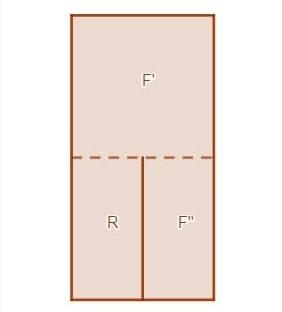
\includegraphics[height=2.3in]{./img1.jpg}
		\end{center}
		\caption{Resultado de dividir $F_i = (w_i \times h_i)$ cuando $w_i < h_i$  \label{fig:1}}%
	\end{figure}
	
	\begin{figure}[htb]%
		\begin{center}
			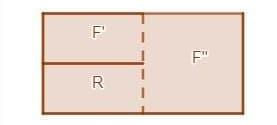
\includegraphics{./img2.jpg}
		\end{center}
		\caption{Resultado de dividir $F_i = (w_i \times h_i)$ cuando $w_i \ge h_i$ \label{fig:2}}%
	\end{figure}

	\item \textbf{DESCSS:} \textit{Sort by Shorter Side First in Descending Order}\\
	Ordenar la entrada $(R_1,...,R_n)$ de acuerdo al siguiente criterio:
	$$R_i < R_j \Longleftrightarrow min(w_i,h_i) < min (w_j,h_j)$$ 
	\item \textbf{RM:} \textit{Rectangle Merge}\\
	La principal limitante del algoritmo es que a causa de mantener una lista de rectángulos libres disjuntos es posible que no permita colocar un rectángulo aún cuando hay suficiente área libre para ello. Una manera en la que se puede mejorar el algoritmo es después de colocar un rectángulo encontrar todos los pares de rectángulos libres vecinos que pueden ser mezclados en uno solo y mezclarlos. Repetir este procedimiento mientras exista al menos un par de rectángulos libres $F_i, F_j$ que cumplan dicha condición.
	
	Se probó el algoritmo tanto con esta heurística como sin ella y de manera general el algoritmo produce mejores salidas aplicando la heurística pero para algunos casos produce una salida peor, por lo que se decidió que a la hora de ejecutar el algoritmo se decide si utilizar o no produciendo un número aleatorio entre 0 y 1. Si ese número es menor que un valor fijo (con 0.75 se obtuvieron buenos resultados) entonces se usa la heurística en esa ejecución del algoritmo. De esta manera se garantiza que se use la heurística en la mayor parte de las ejecuciones del algoritmo pero también permite explorar otras soluciones que solo se obtienen sin usarla y que podrían ser mejores. 
\end{itemize}

En el Algoritmo \ref{guillotine} se muestra un pseudocódigo de la variante de solución propuesta para este problema, incluidas las heurísticas utilizadas. 

 
\algrenewcommand\algorithmicrequire{\textbf{Input:}}
\begin{algorithm}
\caption{Guillotine-BSSF-BFF-SAS-DESCSS-RM}\label{guillotine}
\begin{algorithmic}[1]
	\Require $R \gets \{ R_1 = (w_1 \times h_1), ..., R_n = (w_n \times h_n) \}$ $ M \gets (W \times H)$ \Comment Dimensión de la hoja principal
	\State $F \gets \{(W \times H)\}$
	\State Bins $\gets $ \{ \}
	\State Ordenar R de acuerdo al criterio DESCSS
	\ForAll {$R_k \gets (w_k \times h_k) \in R$}
		\State Elegir rectángulo libre $F_i$ y bin $B_j$ donde colocar $R_k$
		\If {$F_i$, $B_j$ no existen}
			\State Abrir nuevo bin $B$ y a\~nadirlo a Bins
			\State $F \gets F \cup \{(W \times H)\}$
			\State $F_i \gets (W \times H)$
			\State $B_j \gets B$ 
		\EndIf
		\State Decidir orientación del rectángulo
		\State Colocar rectángulo en la esquina inferior izquierda de $F_i$
		\State Dividir espacio sobrante de $F_i$ en $F'$ y $F''$
		\State $F \gets F \cup \{F', F''\} \setminus F_i $
		\While {Existan rectángulos $F_a$ y $F_b$ que se puedan mezclar}
			\State Mezclar $F_a$ y $F_b$ en $F^*$
			\State $F \gets F \cup F^* \setminus \{F_a, F_b\}  $
		\EndWhile
	\EndFor\\
	\Return  Bins
\end{algorithmic}
\end{algorithm}


\subsection{Algoritmo Genético}

Los algoritmos genéticos son llamados así porque se inspiran en la evolución biológica y su base genético-molecular. Estos algoritmos hacen evolucionar una población de individuos sometiéndola a acciones aleatorias semejantes a las que actúan en la evolución biológica (mutaciones y recombinaciones genéticas), así como también a una selección de acuerdo con algún criterio, en función del cual se decide cuáles son los individuos más adaptados, que sobreviven, y cuáles los menos aptos, que son descartados.\cite{5}

El funcionamiento de un algoritmo genético básico se puede resumir en los pasos siguientes:
\begin{itemize}
	\item \textbf{Inicialización}: Se genera aleatoriamente la población inicial, que está constituida por un conjunto de cromosomas los cuales representan las posibles soluciones del problema. En caso de no hacerlo aleatoriamente, es importante garantizar que dentro de la población inicial, se tenga la diversidad estructural de estas soluciones para tener una representación de la mayor parte de la población posible o al menos evitar la convergencia prematura.
	\item \textbf{Evaluación}: A cada uno de los cromosomas de esta población se aplicará la función de aptitud para saber cómo de "buena" es la solución que se está codificando.
	\item \textbf{Condición de término}: El AG se deberá detener cuando se alcance la solución óptima, pero esta generalmente se desconoce, por lo que se deben utilizar otros criterios de detención. Normalmente se usan dos criterios: correr el AG un número máximo de iteraciones (generaciones) o detenerlo cuando no haya cambios en la población. Mientras no se cumpla la condición de término se hace lo siguiente:
	\begin{itemize}
		\item \textbf{Selección}: Después de saber la aptitud de cada cromosoma se procede a elegir los cromosomas que serán cruzados en la siguiente generación. Los cromosomas con mejor aptitud tienen mayor probabilidad de ser seleccionados.
		\item \textbf{Recombinación o cruzamiento}: La recombinación es el principal operador genético, representa la reproducción sexual, opera sobre dos cromosomas a la vez para generar dos descendientes donde se combinan las características de ambos cromosomas padres.
		\item \textbf{Mutación}: Modifica al azar parte del cromosoma de los individuos, y permite alcanzar zonas del espacio de búsqueda que no estaban cubiertas por los individuos de la población actual.
		\item \textbf{Reemplazo}: Una vez aplicados los operadores genéticos, se seleccionan los mejores individuos para conformar la población de la generación siguiente. \cite{5}
	\end{itemize}
\end{itemize}

\subsubsection{Inicialización}\label{init}
Para explicar el proceso seguido a la hora de crear una poblción inicial para el algoritmo lo primero sería definir qué sería el vecindario de una solución. Sea $s \in S$ una solución formada por la configuración $(\pi_1,...,\pi_m)$ correspondiente a $(p_1,...,p_m)$ y $(x_1,...,x_m)$. Un vecino de $s$ se va a construir usando unos de los siguientes operadores: \textit{añadir, eliminar, mover, intercambiar}. 

Sea $L_{max}(i)$ el máximo número posible de hojas de tipo $i$ en un patrón:
$$ L_{max}(i) = \lfloor \frac{H \times W}{h_iw_i} \rfloor$$

Aplicar el operador \textit{añadir} a una solución $s \in S$ añade una hoja $i$ a in patrón $j$ lo que se refleja como un aumento de $p_{ij}$ si $p_{ij} < L_{max}(i)$. El operador \textit{eliminar} consiste en quitar una imagen $i$ del patrón $j$ lo cual disminuye $p_{ij}$ si el número total de hojas $i$ en toda la solución $s$ se matiene estrictamente positivo. El operador \textit{mover} mueve una hoja de un patrón a otro y el operador \textit{intercambiar} intercambia dos hojas entre dos patrones diferentes. 

Un vecino de una solución va a ser generado seleccionando aleatoriamente un operador, uno (\textit{añadir,eliminar}) o dos (\textit{mover, intercambiar}) patrones y una (\textit{añadir,eliminar,mover}) o dos (\textit{intercambiar}) hojas en esos patrones. La aplicación de dichos operadores puede dar como resultado una solución no válida porque sea imposible lograr una configuración para las cantidades $p_j$ obtenidas. Para comprobar la validez de la solución obtenida se utilizó una versión del algoritmo \ref{guillotine}, descrito en la Sección \ref{binpacking}, donde solo va a existir un \textit{bin} disponible y se tratará de construir cada una de las configuraciones solicitadas en la nueva solución, la cual solo pertenecerá a la vecindad de $s$ si este proceso pudo llevarse a cabo exitosamente.      

Para crear la población inicial es necesario generar un conjunto de soluciones válidas. Primero se va a generar una solución $s_0$. Usando el algoritmo \ref{guillotine} solicitando solo una vez cada una de las hojas que se demandan se obtiene las configuraciones $(\pi_1,...,\pi_k)$ y los correspondientes $(p_1,...,p_k)$. Luego resolviendo el problema lineal descrito en la Sección \ref{def} se obtendrían los $(x_1,...,x_k)$ y aplicando la Ecuación \ref{eq3} se asocia a $s_0$ su \textit{fitness}, que es el valor que describe cuán bien cumple el objetivo propuesto. 

Para obtener otra solución a partir de $s_0$ se va a seleccionar una solución $s_1$ que pertenezca al vecinadario de $s_0$ y luego se selecciona una solución $s_2$ que pertenezca al vecinadario de $s_1$ y así sucesivamente hasta que se halla realizado un
número fijo de iteraciones \texttt{NWalk}. Este proceso está encapsulado en la función \textit{RandomWalk(s)}. 

La población inicial va a ser generada aplicando \texttt{NPop} veces la función $RandomWalk(s_0)$. Esto va a constituir la función \textit{CreateInitialPopulation()}.     

\subsubsection{Selección}
En la etapa de selección se utiliza una combinación de dos métodos: Selección Elitista (\textit{Elitist Selection}) y Selección basada en Rango (\textit{Rank Based Selection}).
\begin{itemize}
	\item  \textbf{Selección Elitista:}\\
	Este método consiste en seleccionar los mejores individuos de una población (aquellos con mejores valores de $fitness$) para que formen parte de la próxima generación. En este caso se seleccionan los primeros \texttt{NBest} individuos.
	
	 Este proceso se realiza en la función \textit{ElitistSelection(P)}, donde $P$ es la población de la que se quiere seleccionar los individuos. 
	
	
	\item  \textbf{Selección basada en Rango:}\\
	Este método se basa en un rango que otorga a cada uno de los individuos de la población, de forma que aquel que tenga mejor $fitness$ va a tener rango $n$ mientras que al peor se le otorga rango $1$. La probabilidad de que el individuo $i$ sea seleccionado va a estar dada por la expresión:
	$$ p(i) = \frac{rango(i)}{\sum_{j = 1}^{n}rango(j) } = \frac{rango(i)}{n*(n+1)/2} $$
	
	En el Algoritmo \ref{rank} se presenta el pseudocódigo que describe este método. Este proceso va a estar encapsulado en la función $RankSelection(P)$.
	
	\algrenewcommand\algorithmicrequire{\textbf{Input:}}
	\begin{algorithm}
		\caption{RankSelection}\label{rank}
		\begin{algorithmic}[1]
			\Require $P$
			\State Selección $\gets [\  ]$
			\For {$k \gets 1, \mathtt{NSel}$}
				\State $r \gets Random(0,1)$
				\ForAll {$i \in P$}
					\If {$r < \sum_{j = 1}^{i}p(j)$}
						\State Añadir individuo $i$ a Selección
						\State \textbf{break}
					\EndIf
				\EndFor
			\EndFor \\
			\Return Selección
		\end{algorithmic}
	\end{algorithm}
	  
	
\end{itemize}


\subsubsection{Cruzamiento}\label{cruzamiento}
El cruzamiento es el principal operador genético, el cual va a realizaarse en la función $Crossover(P)$.Se encarga de construir una nueva solución a partir de dos soluciones diferentes que va a escoger de la población $P$. Se escoge un subconjunto de patrones de cada una de las soluciones que serían los padres. El número de patrones escogidos en cada padre va a estar determinado  por un porcentaje del total de patrones del padre que se va a seleccionar aleatoriamente entre 25\% y 50\%. La selección de los patrones va a priorizar aquellos que sean considerados "mejores". La calidad de un patrón va a estar dada por su área libre, la cual mientra menor sea mejor será el patrón. Si existe alguna de las hojas demandadas que no se encuentre en los patrones seleccionados de ambos padres, se construirán nuevos patrones que las incluyan haciendo uso del Algoritmo \ref{guillotine} solicitando una vez cada una de las hojas faltantes. Estos nuevos patrones construidos también van a formar parte de la nueva solución, para la cual a continuación se resolverá el problema de programación lineal descrito en  la Sección \ref{def} y se le asocirán los $(x_1,...,x_m)$  obtenidos así como el valor de $fitness$ correspondiente.

Una vez que se ha obtenido una nueva solución se realiza una mejora de la misma con la función $HillClimbing(s)$. Este proceso va a consistir en buscar una solución $s'$ en el vecindario de $s$, si $s'$ es mejor que que $s$ se repite la búsqueda esta vez en el vecindario de $s'$ y así hasta que la solución vecina no represente una mejora. Para buscar la solución vecina se generan un número fijo de soluciones \texttt{NHill} del vecindario y se selecciona la mejor de estas.     

\algrenewcommand\algorithmicrequire{\textbf{Input:}}
\algrenewcommand\algorithmicensure{\textbf{Inicialización:}}
\begin{algorithm}
	\caption{Crossover}\label{crossover}
	\begin{algorithmic}[1]
		\Require $P$
		\State Offspring $\gets$ \textbf{new} \textit{Solution()}
		\State Parent1 $\gets $ Elegir una solución de $P$
		\State Parent2 $\gets $ Elegir otra solución de $P$
		\State SetPattern1 $\gets $ Elegir patrones de Parent1
		\State SetPattern2 $\gets $ Elegir patrones de Parent2
		\State Añadir $\{$SetPattern1 $\cup$ SetPattern2 $\}$ a Offspring
		\State $R \gets $ Hojas $\notin $ $\{$SetPattern1 $\cup$ SetPattern2
		$\}$
		\State SetPattern3 $\gets Guillotine(R)$ 
		\State Añadir SetPattern3 a Offspring
		\State $ HillClimbing($Offspring$)$\\
		\Return Offspring 
	\end{algorithmic}
\end{algorithm}



\subsubsection{Mutación}

El operador génetico Mutación, como muestra el pseudocódigo en el Algoritmo 	\ref{mutation}, va a seleccionar aleatoriamente un individuo en la población $P$ para que actúe como padre, o sea, como base para formar una nueva solución. Luego se aplica $RandomWalk(s)$ al padre seleccionado como fue explicado en la Sección \ref{init} para crear la población inicial. A continuación se va a mejorar la nueva solución obtenida con $HillClimbing$(Offspring) como fue explicado en la Sección \ref{cruzamiento}.  


\algrenewcommand\algorithmicrequire{\textbf{Input:}}
\begin{algorithm}
	\caption{Mutation}\label{mutation}
	\begin{algorithmic}[1]
		\Require $P$
		\State Parent $\gets $ Elegir una solución de $P$
		\State Offspring $\gets RandomWalk($Parent$)$
		\State $ HillClimbing($Offspring$)$\\
		\Return Offspring 
	\end{algorithmic}
\end{algorithm}


\subsubsection{Algoritmo Principal}
El algoritmo genético que se propone para encontrar una solución al problema de patrones de corte se encuentra resumido en el pseudocódigo que se muestra en el Algotritmo \ref{genetic}. Este es una combinación de las funciones descritas en las secciones anteriores. Se tendrán un total de \texttt{NGen} generaciones y cada una de ellas va a estar compuesta por \texttt{NPop} soluciones. La población de la $k$-ésima generación se va a denotar como $P_k$.

El primer paso sería generar la población inicial $P_0$. Como invariante se tiene que \texttt{BestKnown} va a contener la mejor solución encontrada hasta el momento, la cual se actualiza cada vez que se construye una nueva generación con un llamado a la función $UpdateBestSolution(P)$. Esta función va a seleccionar la mejor solución de $P$. Para cada generación se va a realizar un proceso de selección y de reproducción con los cuales se conformará la próxima generación.

Luego de haber explorado las \texttt{Ngen} generaciones se realizará una mejora a la solución \texttt{BestKnown} haciendo uso de $HillClimbing(\mathtt{BestKnown})$.
 
\algrenewcommand\algorithmicrequire{\textbf{Input:}}
\algrenewcommand\algorithmicensure{\textbf{Inicialización:}}
\begin{algorithm}
	\caption{GeneticAlgorithm}\label{genetic}
	\begin{algorithmic}[1]
		\State $P_0 \gets CreateInitialPopulation()$
		\State BestKnown $\gets UpdateBestSolution(P_0)$
		\For {$k \gets 1, \mathtt{NGen}$}
		\State$P_{k-1}^* \gets RankSelection(P_{k-1})$
		\State$P_{k} \gets ElitistSelection(\mathtt{NBest},P_{k-1})$
			\For {$i \gets \mathtt{NBest}+1, \mathtt{NPop}$}
				\If {$Random(0,1) < \mathtt{ProbCross}$}
					\State Añadir $Crossover(P_{k-1}^*)$ a $P_k$
				\Else
					\State Añadir $Mutation(P_{k-1}^*)$ a $P_k$
				\EndIf	
			\EndFor
		\State BestKnown $\gets UpdateBestSolution(P_k)$
		\EndFor
		\State $ HillClimbing($BestKnown$)$\\
		\Return BestKnown
	\end{algorithmic}
\end{algorithm}


\subsubsection{Ajuste de Parámetros}
El algoritmo génetico precisa de varios parámetros para su funcionamiento. Según cúan adecuados sean estos parámetros para el problema en cuestión mejores serán los resultados obtenidos. Por tanto se necesita determinar que valores asignarle a \texttt{NWalk, Ngen, NPop, NBest, NSel, NHill} y \texttt{ProbCross}.
Para lograr este objetivo se recurrió a la experimentación y observación de los resultados y después de explorar varias combinaciónes de parámetros se encontró que los mejores resultados se alcanzaban con la siguiente configuración: \texttt{NWalk =} 100, \texttt{Ngen =} 30, \texttt{NPop =} 60, \texttt{NBest =} 10, \texttt{NSel =} 45, \texttt{NHill =} 25 y \texttt{ProbCross =} 0.75.

Para mostrar el desempe\~no de la configuración de los par\'ametros anterior se resolvieron un total de 50 instancias diferentes del problema, donde se solicitan desde 1 hasta 12 tipo de hojas diferentes y las demandas de estas llegan a alcanzar cantidades cercanas al mill\'on. Como resultados se reporta que el mayor tiempo requerido para hallar la soluci\'on fue de 169 segundos, mientras que el tiempo promedio fue de 25 segundos. Se observ\'o adem\'as que los casos en que m\'as demoraba eran aquellos en los que las dimensiones de la hoja principal eran grandes y las dimensiones de las hojas solicitadas eran peque\~nas.    

\section{Interfaz Visual}\label{visual}
Para poder hacer uso de la solución propuesta se provee una aplicación de escritorio desarrollada con \texttt{PyQt5} como herramienta. Esta brinda una interfaz visual al usuario para introducir una instancia del problema a resolver.

% Conclusiones
%-----------------------------------------------------------------------------------
\section{Conclusiones}\label{sec:conc}
En este proyecto se resolvi\'o un problema de patrones de cortes relacionado a la industria del papel. La solución propuesta se basa en un problema de programación lineal, un problema de empaquetamiento y un algoritmo génetico. Como trabajo futuro se recomienda tratar de encontrar combinaciones de par\'ametros del algoritmo gen\'etico que proporcionen mejores resultados, as\'i como probar otras estrategias de selecci\'on.  

 Los resultados obtenidos fueron satisfactorios pues se logr\'o automatizar un proceso que se realiza de forma manual. Si se usa la aplicaci\'on propuesta se podr\'ia agilizar potencialmente el trabajo diario en la empresa pues se obtendr\'ian resultados que minimizan el desperdicio en cuesti\'on de pocos minutos. 


%===================================================================================

%===================================================================================
\renewcommand{\refname}{Referencias Bibliogr\'aficas}
% Bibliografía
%-----------------------------------------------------------------------------------
\begin{thebibliography}{99}
%-----------------------------------------------------------------------------------	


	\bibitem{51} Ben Lagha, G.a , Dahmani, N.b , Krichen, S.a.
	Particle swarm optimization approach for resolving the
	cutting stock problem. 2014 International Conference
	on Advanced Logistics and Transport, 2014.
	
	\bibitem{41}  Cui, Y.-P., Tang, T.-B. Parallelized sequential value correction procedure for the one-dimensional cutting
	stock problem with multiple stock lengths. Engineering
	Optimization, 46 (10), 1352-1368, 2014.
	
	\bibitem{48}  Díaz, D., Valledor, P., Areces, P., Rodil, J., Suárez, M.
	An ACO Algorithm to Solve an Extended Cutting Stock
	Problem for Scrap Minimization in a Bar Mill. Lecture
	Notes in Computer Science (including subseries Lecture
	Notes in Artificial Intelligence and Lecture Notes in
	Bioinformatics), 8667, 13-24, 2014.
	
	\bibitem{2} H. Hideki, and M.J. Pinto, “An integrated cutting
	stock and sequencing problem,” European Journal of
	Operational Research (183), 1353–1370, 2007.
	
	\bibitem{11} J. Jylanki. A thousand ways to pack the bin - a
	practical approach to two-dimensional rectangle bin
	packing. research report, 2010.
	
	\bibitem{3}J. Karelahti, “Solving the cutting stock problem in
	the steel industry”. Department of Engineering Physics
	and Mathematics. Helsinki University of Technology,
	2-5, 2002.
	
	\bibitem{46}  Lu, H.-C.a , Huang, Y.-H.b. An efficient genetic
	algorithm with a corner space algorithm for a cutting
	stock problem in the TFT-LCD industry. European
	Journal of Operational Research, 246 (1), 51-65, 2015.
	
	\bibitem{47}Lu, Q., Zhou, X. GPU parallel ant colony algorithm
	for the dynamic one-dimensional cutting stock problem
	based on the on-line detection. Yi Qi Yi Biao Xue Bao/
	Chinese Journal of Scientific Instrument, 36 (8), pp.
	1774-1782, 2015.
	
	\bibitem{42} MirHassani, S.A., Jalaeian Bashirzadeh, A. A
	GRASP meta-heuristic for two-dimensional irregular
	cutting stock problem. International Journal of
	Advanced Manufacturing Technology, 81 (1-4), 455-
	464, 2105.
	
	\bibitem{1} P. Gilmore, and R. Gomory, “A linear programming
	approach to the Cutting Stock Problem-Part II,”
	Operations Research, 11(6), 863-888, 1963.
	
	\bibitem{29} R. Haessler, and P. Sweeney, “Cutting stock
	problems and solution procedures,” European Journal
	of Operational Research, 54, 141-150, 1991.
	
	\bibitem{4} Stéphane Bonnevay, Philippe Aubertin, and Gérald Gavin, "A Genetic Algorithm to Solve a Real 2-D Cutting Stock
	Problem with Setup Cost in the Paper Industry". Genetic and Evolutionary Computation Conference,2015
	
	\bibitem{43}  Wenshu, L., Dan, M., Jinzhuo, W. Study on cutting
	stock optimization for decayed wood board based
	on genetic algorithm. Open Automation and Control
	Systems Journal, 7 (1), 284-289, 2015.
	
	\bibitem{5} Wikipedia. URL: \href{https://es.wikipedia.org/wiki/Algoritmo\_genetico}
	{https://es.wikipedia.org/wiki/ \\Algoritmo\_genetico}.
	Consultado el 1 de Noviembre, 2020.

%-----------------------------------------------------------------------------------
\end{thebibliography}

%-----------------------------------------------------------------------------------

\label{end}
\end{hyphenrules}
\end{document}

%===================================================================================
